\section{Level and flow control loop}

Interactive level and flow control necessitates the use of multivariable control techniques.  Figure~\ref{fig:rig:levelflow} shows the rig used for this application.  Dead time can be incorporated by using a dead time pan. 
\begin{figure}
	\centering
	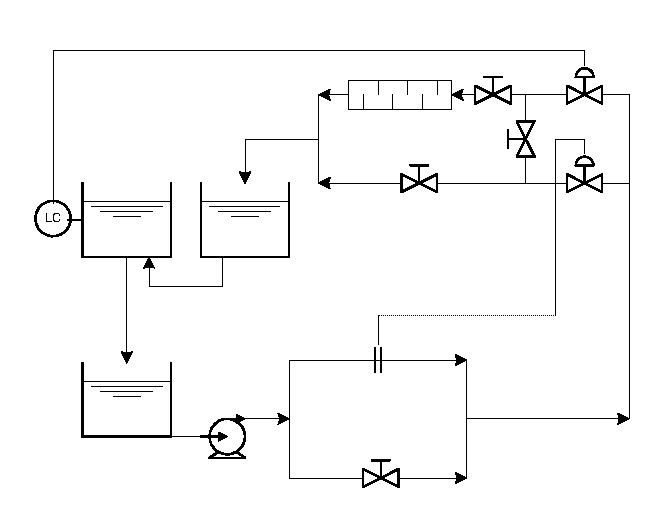
\includegraphics{LevelFlow}
	\caption{The level and flow control loop}
	\label{fig:rig:levelflow}
\end{figure}
The robust nature of the rig makes it ideal for the implementation and development of advanced analysis and control techniques like on-line tuning and fault detection.  Contemporary control techniques such as fuzzy logic or neural network control can also be attempted, as the system dynamics are straightforward and easily checked.

%\subsection{Procedures}

%\subsubsection{Commissioning}

%\subsubsection{Startup}

%\subsubsection{Shutdown}

%\subsubsection{Decommissioning}
